\documentclass{beamer}
\usepackage[utf8]{inputenc}
\usepackage{tikz}
\usetikzlibrary{arrows}
% Declare layers
%\usetheme{Madrid}
%\usecolortheme{seahorse}
%Information to be included in the title page:
\title[CSCI 6676 - Numerical Optimization]{CSCI 6676 - Numerical Optimization}
\author{Nilesh Jagnik}
\institute[CU Boulder]{University of Colorado Boulder}
\date{April 25th, 2016}

%------------------------------------------------------------
\addtobeamertemplate{navigation symbols}{}{%
    \usebeamerfont{footline}%
    \usebeamercolor[fg]{footline}%
    \hspace{1em}%
    \insertframenumber/\inserttotalframenumber
}
%------------------------------------------------------------
\begin{document}
\frame{\titlepage}










%--------------COPY BELOW THIS LINE-------------------------










%---------------------------------------------------------
\begin{frame}
\frametitle{\centerline{Calculating Derivatives - Finite Difference}}
Approximate derivative at a point $x$ by observing change in function values in response to small perturbations of the unknown near $x$.\\
\hfill \break
\hfill \break
\centerline{$\frac{\partial f}{\partial x_i} \approx \frac{f(x+\epsilon e_i)-f(x+\epsilon e_i)}{2\epsilon}$}
\hfill \break
Where $\epsilon$ is a small scalar and $e_i$ is the $i$th unit vector. 
\end{frame}
%---------------------------------------------------------
\begin{frame}
\frametitle{\centerline{Approximating The Gradient - Forward Difference}}
%\centerline{$f(x+\epsilon e_i) = f(x) + \epsilon \frac{\partial f}{\partial x_i} + \frac{1}{2}\epsilon^2 \frac{\partial^2 f}{\partial^2 x_i} + O(\epsilon^3)$}
\centerline{$f(x+\epsilon e_i) = f(x) + \epsilon \frac{\partial f}{\partial x_i} + O(\epsilon^2)$}
\hfill \break
\hfill \break
\centerline{$\frac{\partial f}{\partial x_i}(x) = \frac{f(x+\epsilon e_i)-f(x)}{\epsilon} + O(\epsilon)$}
\end{frame}
%---------------------------------------------------------
\begin{frame}
\frametitle{\centerline{Approximating The Gradient - Central Difference}}
\centerline{$f(x+\epsilon e_i) = f(x) + \epsilon \frac{\partial f}{\partial x_i} + \frac{1}{2}\epsilon^2 \frac{\partial^2 f}{\partial^2 x_i} + O(\epsilon^3)$}
\centerline{$f(x-\epsilon e_i) = f(x) - \epsilon \frac{\partial f}{\partial x_i} + \frac{1}{2}\epsilon^2 \frac{\partial^2 f}{\partial^2 x_i} + O(\epsilon^3)$}
\hfill \break
\hfill \break
\centerline{$\frac{\partial f}{\partial x_i} \approx \frac{f(x+\epsilon e_i)-f(x+\epsilon e_i)}{2\epsilon} + O(\epsilon^2)$}
\end{frame}
%---------------------------------------------------------
\begin{frame}
\frametitle{\centerline{Accuracy And Cost}}
The error in central-difference method is $O(\epsilon^2)$ as compared to $O(\epsilon)$ in forward-difference method. This is desirable because numerical calculations do not work very well when $\epsilon$ is too small.\\
\hfill \break
\hfill \break
Central-difference method is costly and requires two additional function evaluations. In practice, there are errors in these function evaluations and the accuracy is not worth the additional cost. 
\end{frame}
%---------------------------------------------------------
\begin{frame}
\frametitle{\centerline{Jacobian}}
The Jacobian of a vector function $r:\mathbb{R}^n \rightarrow \mathbb{R}^m$ is defined as :\\
\hfill \break
\begin{equation*}
\mathbf{J}(x) = \left(
\begin{array}{ccc}
\frac{\partial r_1}{\partial x_1} & \ldots & \frac{\partial r_1}{\partial x_n}  \\
\vdots & \ddots & \vdots \\
\frac{\partial r_m}{\partial x_1} & \ldots & \frac{\partial r_m}{\partial x_n}  \\
\end{array} \right)
= \left(
\begin{array}{ccc}
\nabla r_1(x)^T \\
\nabla r_2(x)^T \\
\vdots\\
\nabla r_m(x)^T \\
\end{array} \right)
\end{equation*}
\end{frame}
%---------------------------------------------------------
\begin{frame}
\frametitle{\centerline{Approximating Jacobian using FD}}
We use the finite difference method to derive the following estimate of the $i$th column:\\
\hfill \break
\hfill \break
\centerline{$\frac{\partial r}{\partial x_i}(x) = \frac{r(x+\epsilon e_i)-r(x)}{\epsilon}$}
\hfill \break
\hfill \break
A full Jacobian can be obtained at a cost of $n+1$ function evaluations.
\end{frame}
%---------------------------------------------------------
\begin{frame}
\frametitle{\centerline{Approximating Sparse Jacobian}}
However, when the matrix is sparse, we can often obtain the estimate at much lower cost.\\
\hfill \break
\hfill \break
The key is to chose points in a way that they may be used to estimate multiple columns.\\
\hfill \break
\hfill \break
For example, instead of chosing to perturb in direction $p =\epsilon e_i$, we chose $p = \epsilon(e_i+e_j)$ when $x_i$ and $x_j$ are \textit{not present in the same component of $r$}. 
\end{frame}
%---------------------------------------------------------
\begin{frame}
\frametitle{\centerline{Example}}
\begin{equation*}\label{eq:8.13} \tag{8.13}
r(x) = \left(
\begin{array}{ccc}
2(x_2^3-x_1^2) \\
3(x_2^3-x_1^2) + 2(x_3^3 - x_2^2)\\
3(x_3^3-x_2^2) + 2(x_4^3 - x_3^2)\\
3(x_4^3-x_3^2) + 2(x_5^3 - x_4^2)\\
3(x_5^3-x_4^2) + 2(x_6^3 - x_5^2)\\
3(x_6^3-x_5^2)\\
\end{array} \right)
\end{equation*}
\end{frame}
%---------------------------------------------------------
\begin{frame}
\frametitle{\centerline{Jacobian Structure for $r(x)$}}
\begin{equation*}
J(x) = \left(
\begin{array}{cccccc}
\times & \times & & & &\\
\times & \times & \times & & & \\
&\times & \times & \times & &\\
& &\times & \times & \times &\\
& & &\times & \times & \times\\
& & & & \times & \times\\
\end{array} \right)
\end{equation*}
\hfill \break
\hfill \break
$1$st column and $4$th column have no overlap. $x_1$ and $x_4$ can be perturbed by a single point.
\end{frame}
%---------------------------------------------------------
\begin{frame}
\frametitle{\centerline{Perturbation Vectors}}
We chose\\
\centerline{$p = \epsilon(e_1 + e_4)$}
\hfill \break
\hfill \break
and note that\\
\centerline{$r(x+p)_{1,2} = r(x + \epsilon(e_1 + e_4))_{1,2} = r(x + \epsilon(e_1))_{1,2}$}
\hfill \break
\hfill \break
\centerline{$r(x+p)_{3,4,5} = r(x + \epsilon(e_1 + e_4))_{3,4,5} = r(x + \epsilon(e_4))_{3,4,5}$}
\end{frame}
%---------------------------------------------------------
\begin{frame}
\frametitle{\centerline{Estimating Multiple Columns With Single Fn Evaluation}}
Using $p = \epsilon(e_1 + e_4)$, we can write:\\
\hfill \break
For Column 1,\\
\begin{equation*}
\left(
\renewcommand{\arraystretch}{1.5}
\begin{array}{c}
\frac{\partial r_1}{\partial x_1}(x)\\
\frac{\partial r_2}{\partial x_1}(x)\\
\end{array} \right)
\approx \frac{r(x+p)_{1,2} - r(x)_{1,2}}{\epsilon}
\end{equation*}
\hfill \break
\hfill \break
For Column 4,\\
\begin{equation*}
\left(
\renewcommand{\arraystretch}{1.5}
\begin{array}{c}
\frac{\partial r_4}{\partial x_3}(x)\\
\frac{\partial r_4}{\partial x_4}(x)\\
\frac{\partial r_4}{\partial x_5}(x)\\
\end{array} \right)
\approx \frac{r(x+p)_{3,4,5} - r(x)_{3,4,5}}{\epsilon}
\end{equation*}
\end{frame}
%---------------------------------------------------------
\begin{frame}
\frametitle{\centerline{Reduction of Function Evaluations}}
Similarly, for columns 2 and 5:\\
\centerline{$p_2 = \epsilon(e_2 + e_5)$}
\hfill \break
\hfill \break
And for columns 3 and 6:\\
\centerline{$p_3 = \epsilon(e_3 + e_6)$}
\hfill \break
\hfill \break
Instead of using six function evaluations, we only use three.
\end{frame}
%---------------------------------------------------------
\begin{frame}
\frametitle{\centerline{Reduction to Graph Coloring}}
For any function $r:\mathbb{R}^n \rightarrow \mathbb{R}^m$, we can construct a column incident graph by drawing an edge between nodes $i$ and $k$ if there is some component of $r$ that depends on both $x_i$ and $x_k$.\\
\hfill \break
\hfill \break
We assign each node a color using the following rule: Two nodes can have the same color if there is no edge that connects them.\\
\hfill \break
\hfill \break
If nodes $i_1,i_2....i_l$ have the same color, the correspoding perturbation vector is $p = \epsilon(e_{i_1} + e_{i_2} + .... + e_{i_l})$.\\
%\ref{eq:8.13}
\end{frame}
%---------------------------------------------------------
\begin{frame}
\frametitle{\centerline{Graph For $r(x)$}}
\begin{figure}[!h]
\centering
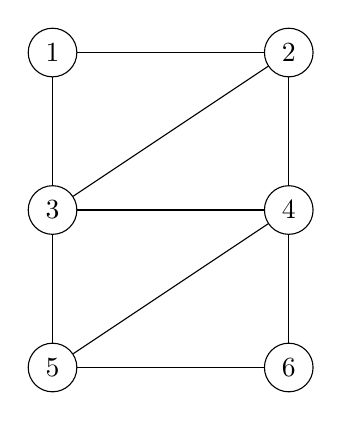
\begin{tikzpicture}

\tikzset{vertex/.style = {shape=circle,draw,minimum size=1.5em}}
\tikzset{edge/.style = {}}
% vertices
\node[vertex] (1) at  (0,2) {$1$};
\node[vertex] (2) at  (3,2) {$2$};
\node[vertex] (3) at  (0,0) {$3$};
\node[vertex] (4) at  (3,0) {$4$};
\node[vertex] (5) at  (0,-2) {$5$};
\node[vertex] (6) at  (3,-2) {$6$};
%edges
\draw[edge] (1) to (2);
\draw[edge] (2) to (3);
\draw[edge] (1) to (3);
\draw[edge] (2) to (4);
\draw[edge] (3) to (4);
\draw[edge] (3) to (5);
\draw[edge] (4) to (5);
\draw[edge] (4) to (6);
\draw[edge] (5) to (6);
\end{tikzpicture}
\caption{Column Index graph for $r(x)$ defined in \ref{eq:8.13}}
\end{figure}
\end{frame}
%---------------------------------------------------------
\begin{frame}
\frametitle{\centerline{Performance of Coloring Algorithms}}
Finding optimal coloring requires exponential time.\\
\hfill \break
\hfill \break
There are faster algorithms that find near-optimal solutions.\\
\hfill \break
\hfill \break
A greedy algorithm - Start by giving a color to node with highest degree. And eliminate possibilities.
\end{frame}



%-------------COPY ABOVE THIS LINE------------------------














%---------------------------------------------------------
\end{document}
